\documentclass{article}

\usepackage{amssymb,amsmath,amsfonts,amstext}
\usepackage{graphicx}
%\usepackage{subfigure}
\usepackage{mathtools}
\usepackage{stmaryrd}
\usepackage{color}
\usepackage{verbatim}
\usepackage{amsthm}
\usepackage{esint}
\usepackage{caption,subcaption}
\usepackage{titlesec}
\setcounter{secnumdepth}{4}
\usepackage{geometry}
\geometry{left=3.18cm,right=3.18cm,top=2.54cm,bottom=2.54cm}


\title{Recurrent neural network}
\author{Xiaoguai Li}
\date{}

\begin{document}


\maketitle
Train recurrent neural network to predict
\begin{equation}\nonumber
f=\sin(\pi t)+\sin(\pi/2.0*t)+\sin(\pi/4.0*t)
\end{equation}\
for $t \in [0, 100]$.
Figure.1 is obtained from RNN\_timeSequence.py. The long short-term memory networks are realized in LSTM.py. The test interval is $[66.5,100]$. The L2 norm error of following plot is 6.94666\%.
\begin{figure}[h]
    \center
    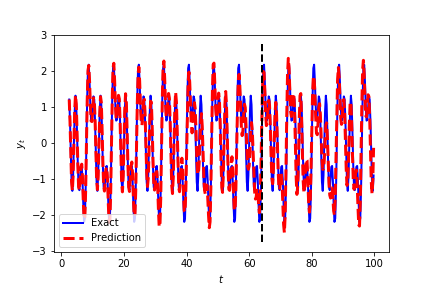
\includegraphics[width=0.6\textwidth]{prediction}
    \caption{Prediction and exact values at different time}
\end{figure}


\end{document}



